\documentclass[12pt, a4paper]{article} %mostra o tipo do documento
\setlength{\topmargin}{-.5in}
\setlength{\textheight}{9in}
\setlength{\textwidth}{6.3in}
\setlength{\oddsidemargin}{-.125in}
\setlength{\evensidemargin}{-.125in}
\usepackage[brazil]{babel} %permite escrever em português
\usepackage[utf8]{inputenc}
\usepackage[a4paper, textheight=260mm, textwidth=162mm]{geometry} %ajusta as margens
\usepackage[T1]{fontenc} %define a fonte das letras
\usepackage{color} %colore as letras
\usepackage{url} %inclui urls
\usepackage[pdfencoding=unicode]{hyperref} %transforma links em texto comum para clicar
\usepackage{amsmath, amssymb, amsthm, amsfonts} %permite fazer textos matemáticos
\usepackage{float} % permite mover tabelas e figuras para qualquer ponto da página
\usepackage{graphicx} %permite colocar imagens no documento

\title{Relatório EP2 - MAC0121}
\date{}
\author{João Gabriel Basi - $\text{N}^\circ$ USP: 9793801}
\begin{document}
\maketitle
\begin{enumerate}
\large
\item[1.]\textbf{O programa}
\normalsize\\[0.5cm]
Utiliza a técnica de backtracking para achar uma solução para o jogo de tabuleiro "Resta Um". O programa recebe as dimenções do tabuleiro e um matriz com 0, -1 e 1, representando "sem buraco", "buraco sem peça" e "buraco com peça" respectivamente, e retorna os movimentos realizados para resolver o tabuleiro ou "Impossivel" se não há como resolvê-lo.\\
\large
\item[2.]\textbf{As funções}
\normalsize\\[0.5cm]
Foi criada uma struct pilha que contém um vetor de triplas (a posição da peça e o movimento executado), além de variávies para o topo da pilha e seu tamanho máximo.\\
Foram criadas também algumas funções sobre essa struct:
\begin{itemize}
\item $criaPilha$: Aloca uma pilha de número de linhas especificado;
\item $pilhaVazia$: Verifica se a pilha está vazia;
\item $pilhaCheia$: Verifica se a pilha está cheia;
\item $empilha$: Empilha uma posição e um movimento na pilha;
\item $desempilha$: Desempilha a posição e o movimento que estão no topo da pilha;
\item $imprimePilha$: Imprime as posições de início e fim de cada movimento guardado na pilha;
\item $freePilha$: Desaloca uma pilha.
\end{itemize}
Foram criadas funções para ajudar na manipulação de matrizes e vetores:
\begin{itemize}
\item $criaVetor$: Aloca um vetor de tamanho especificado;
\item $criaMatriz$: Aloca uma matriz de número de linhas e colunas especificados;
\item $podeMexer$: Verifica se a peça pode ser movida e indica a direção do movimento;
\item $mexe$: Executa ou volta um movimento;
\item $freeMatriz$: Desaloca uma matriz.
\end{itemize}
E foram criadas algumas funções para verificações sobre matrizes:
\begin{itemize}
\item $concluido$: Verifica se as posições que estavam livres no começo estão ocupadas;
\item $ehPossivel$: Faz alguns testes (especificados no item 3) na distribuição das peças do tabuleiro para filtrar alguns tabuleiros insolúveis;
\item $floodFill$: Utilizada pela função $ehPossivel$ para verificar se o tabuleiro tem partes desconexas;
\item $criaPagoda$: Cria uma matriz seguindo alguns parâmetros simples para a verificação da função $checaPagoda$;
\item $checaPagoda$: Checa se o valor da função pagoda do tabuleiro atual é maior que o valor do tabuleiro final (mais detalhes no item 3).
\end{itemize}
\large
\item[3.]\textbf{Conceitos matemáticos e simplificações utilizados}
\normalsize\\[0.5cm]
Na função $ehPossivel$ foram feitos três testes para identificar se um tabuleiro tem potencial para ser resolvido:
\begin{itemize}
\item O primeiro teste checa se $\text{N}^\circ$ de peças $\geqslant 2\cdot \text{N}^\circ$ de espaços iniciais, pois, para cada buraco sem peça do tabuleiro inicial é preciso de, no mínimo, um movimeto, e cada movimento precisa de duas peças para ser executado, então, se o tabuleiro tem $n$ buracos, é preciso de, pelo menos, $2n$ peças para resolvê-lo.
\item O segundo teste leva em conta a classe de posições do tabuleiro. Conforme foi descrito no site Recmath\cite{recmath}, a classe de posições do tabuleiro é definida enumerando as diagonais do tabuleiro do seguinte modo:\\
\small
\begin{center}
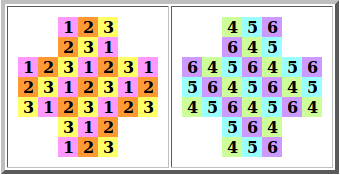
\includegraphics[scale=0.5]{peg_solitaire_classes.png}\\
Numeração no resta um tradicional\cite{recmath}\\
\end{center}
\normalsize
A partir disso, definimos uma função $N_i$ sobre o tabuleiro, que retorna a quantidade de casas ocupadas marcadas com número $i$, e a função $T$, que retorna o total de casas ocupadas. Com isso definimos a classe de posições do tabuleiro como sendo a 6-upla da forma $(T-N_1,T-N_2,T-N_3,T-N_4,T-N_5,T-N_6)\text{ }mod\text{ }2$ (no site é colocado como a "paridade" desses números, mas no programa eu considerei como módulo 2). Definidas as classes, observamos que a cada movimento executado a paridade dos númes dessa 6-upla não muda. Pegando como exemplo o tabuleiro da imagem, com a posição central livre e as outras ocupadas, vemos que, ao mexer qualquer peça para a posição central, os $N_2$ e $N_5$ aumentam em $1$ e os $N_1$, $N_3$, $N_4$, $N_6$ e $T$ diminuem em $1$, então, para os $N$s que diminuiram, temos que $N-1-(T-1)\equiv N-T\text{ }mod\text{ }2$, e para os que aumentaram $N+1-(T-1)\equiv N-T\text{ }mod\text{ }2$, vemos que essa regra vale para todo o tabuleiro e, concluimos que, a partir de um tabuleiro com certa classe de posição, só é possível atingir tabuleiros com a mesma classe, então temos que os tabuleiros final e inicial têm que estar na mesma classe, se não o tabuleiro é impossível. Lembrando que esse teste indicar que um tabuleiro é impossível é suficiente para que ele seja impossível, mas não é necessário.
\item O terceiro leva em conta a possibilidade de tabuleiros com partes desconexas, checando com a função $floodFill$ se, sempre quando há uma parte desconexa, ela tem no mínimo uma casa vazia, para que todas as peças possam ser movidas.\\[-0.5cm]
\end {itemize}
Outra simplificação utilizada foi uma fução contadora de recursos (também chamada de Pagoda) introduzida pela primeira vez no volume 4 do livro "Winning ways for your mathematical plays". Para calcular a função temos que atribuir um valor de forma estratégica para cada casa do tabuleiro. O valor da função em um determinado tabuleiro é a soma dos valores das casas ocupadas. Como os valores das casas não são negativos e uma peça sempre é retirada do tabuleiro por movimento, o valor da função não pode aumentar, portanto, se o valor do tabuleiro atual for menor que o valor do tabuleiro final, o conjunto de movimentos executados não resolverá o jogo.\\
\small
\begin{center}
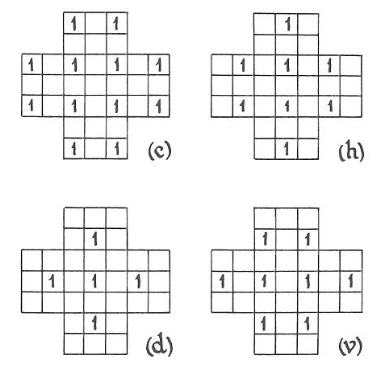
\includegraphics[scale=0.5]{pagoda.png}\\
Exemplos de funções Pagoda\cite{wwmp}\\
\end{center}
\normalsize
A imagem acima mostra algumas funções que podem ser utilizadas quando há somente um buraco no tabuleiro. Para uma melhor estratégia de jogo, escolhemos a função que tem o número $1$ marcado no lugar em que há um buraco, assim, forçamos o valor do tabuleiro final a ser $1$. Com isso, se retirarmos todas as peças que ocupam as casas de valor $1$, não há mais peças que conseguem chegar na posição do buraco inicial, por isso, o valor da função nesse estado de jogo é $0$, então sabemos que nenhum movimento adicional pode concluir o jogo.\\
No programa, a função $criaPagoda$ produz um dos tabuleiros da imagem ou a junção de dois ou mais tabuleiros diferentes, dependendo das posições dos buracos iniciais, e a $checaPagoda$ verifica se o valor da função no tabuleiro atual não é menor que o do tabuleiro final.\\
\small
\begin{center}
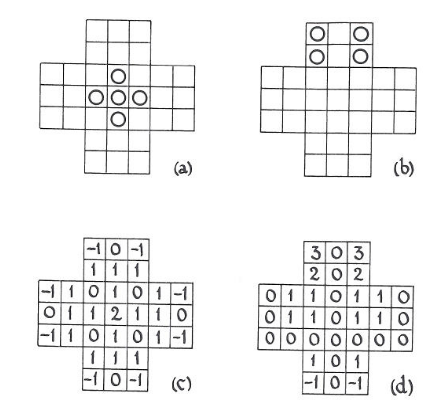
\includegraphics[scale=0.5]{pagoda2.png}\\
Funções Pagoda de dois tabuleiros\\
(os círculos representam as casas vazias do começo)\cite{wwmp}
\end{center}
\normalsize
Qualquer tabuleiro preenchido com valores que obedecem as condições da função pode ser utilizado, porém não há um algoritmo rápido para gerar esses tabuleiros mais "personalizados", como os da figura acima (ao menos eu não achei nenhum), por isso, o programa produz tabuleiros simples que também funcionam, mas não são os melhores.\\
%Peguemos como exemplo o tabuleiro $(d)$ da imagem acima. Para o jogo que começa com o buraco no centro do tabuleiro, a estratégia da figura é que tem que haver ao menos uma peça em alguma das casas marcadas com $1$, pois se não houver nenhuma não há como levar uma peça ao buraco central no final do jogo. Para um buraco qualquer, é só selecionar o tabuleiro acima que tem a casa inicialmente vazia marcada com 1, e aplicar a regra de que o valor da função não pode aumentar.\\
\large
\item[4.]\textbf{Informações sobre os testes realizados}
\normalsize\\[0.5cm]
Considerando como núcleo a formação $3$x$3$ central do tabuleiro tradicional (imagem do item anterior) com a posição central livre e as outras ocupadas, e como braços as quatro partes restentes, escrevemos que um tabuleiro é $nnnn$ se tem o núcleo e $4$ braços $3$x$n$, contados a partir do de cima em sentido horário (notação encontrada no site citado no item 3).\\
\begin{itemize}
\item Testei com um tabuleiro $1111$, que passou nos testes da $ehPossivel$, mas, depois de $140seg$ (sem otimização o programa demorou o mesmo tempo), o programa concluiu que ele é impossível;
\item Testei para um tabuleiro $1111$ com o buraco central e mais dois opostos e adjacentes a ele, que o programa concluiu que é impossivel em $4seg$ (sem otimização o programa demorou $25 seg$);
\item Testei com o tabuleiro $2222$ e um $6$x$4$ (só esse com um buraco em qualquer lugar), que ele resolveu em pouco menos de $1seg$ (mesmo tempo do programa sem otimização);
\item Testei para um $2121$, que ele resolveu em $130seg$.
\item Testei com um tabuleiro $3322$, que passou no teste da $ehPossivel$, mas o programa não consiguiu achar uma resolução depois de meia hora rodando;
\item Testei para o tabuleiro francês, um tabuleiro com um núcleo $5$x$5$, e $4$ braços $3$x$1$ (também descrito em \cite{recmath}) e o programa concluiu, ainda no teste das classes, que esse tabuleiro não é possível;
\item Testei com o tabuleiro $3333$, que não foi resolvido depois de 3 horas.\\[0.5cm]
\end{itemize}
\large
\item[5.]\textbf{Prós e contras}
\normalsize\\[-0.5cm]
\begin{itemize}
\item \textbf{Prós}\\[-0.5cm]
\begin{itemize}
\item Identifica boa parte dos tabuleiros que são impossíveis no começo do programa, deixando de gastar tempo tentando resolvê-los;
\item A função Pagoda melhora o desempenho do programa.
\end{itemize}
\item \textbf{Contras}
\begin{itemize}
\item Mesmo utilizando a função Pagoda, alguns tabuleiros com mais de quatro buracos não podem ser otimizados pelo algoritmo desse programa, pois a função Pagoda gerada é uma versão simplificada e não abrange muitos casos.  
\end{itemize}
\end{itemize}
\end{enumerate}
\begin{thebibliography}{3}
\bibitem{recmath} Imagens retiradas do site \url{http://recmath.org/pegsolitaire/index.html#pre}
\bibitem{wwmp} Imagens retiradas do livro "Winning ways for your mathematical plays" vol. 4
/\end{thebibliography}
\end{document}